\documentclass[tikz, border=5mm]{standalone}
\usepackage{textcomp}
\usetikzlibrary{arrows.meta,decorations.markings,fit,calc, positioning}

\definecolor{componentColor}{RGB}{210,210,210}
\definecolor{systemColor}{RGB}{230,230,230}

\tikzset{component/.append style={fill=componentColor, align=center, draw, minimum width=2cm, minimum height=1.5cm, rounded corners=.3cm,node distance=0.8cm and 1.5cm}}
\tikzset{system/.style={component, fill=systemColor, rounded corners=0cm}}
\tikzset{interface/.style={system, fill=systemColor, minimum size=1.6cm}}


\begin{document}

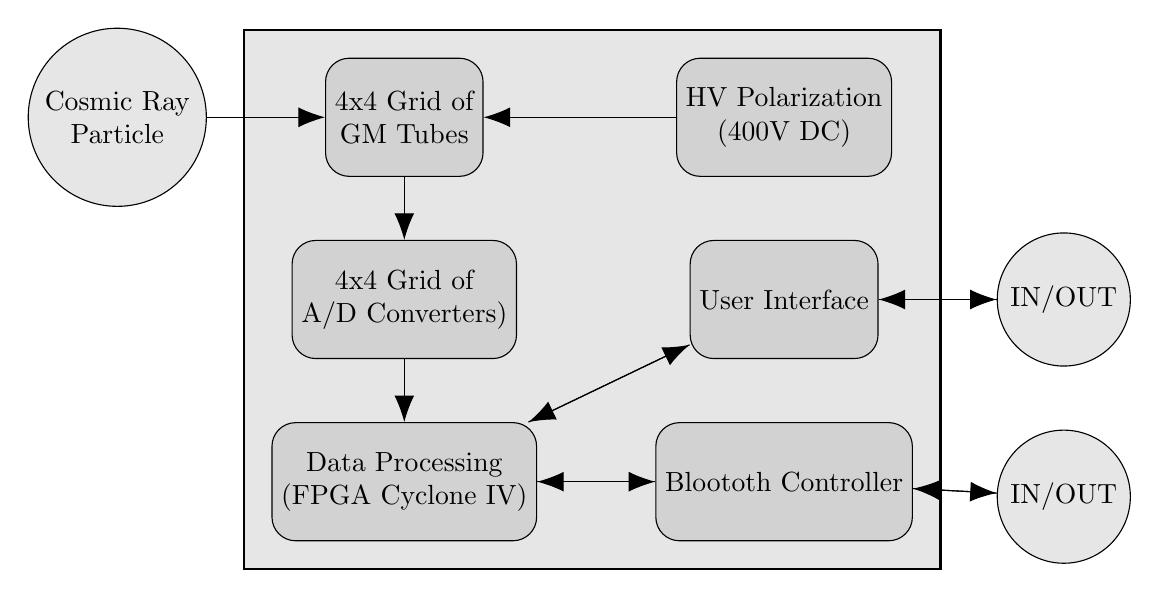
\begin{tikzpicture}[node distance=1.5cm and 3cm]
% Nodes
\pgfdeclarelayer{background}
\pgfsetlayers{background,main}

    \node (CosmicRayParticle) [circle, interface] {Cosmic Ray\\ Particle};

    \node (GMTubes) [component, right=of CosmicRayParticle] {4x4 Grid of\\ GM Tubes};


    \node (ADConverters) [component, below=of GMTubes] {4x4 Grid of\\ A/D Converters)};

    \node (GMDataProcessing) [component, below=of ADConverters] {Data Processing\\ (FPGA Cyclone IV)};

    \node (BlootothController) [component, right=of GMDataProcessing] {Bloototh Controller};

    \node (UserInterface) [component, above=of BlootothController] {User Interface};

    \node (PolarizationVoltage) [component, above=of UserInterface] {HV Polarization\\ (400V DC)};


    \node (UserInterface_InOut) [circle, interface, right=of UserInterface] {IN/OUT};

    \node (BlootothController_InOut) [circle, interface, below=of UserInterface_InOut] {IN/OUT};

\begin{pgfonlayer}{background}
\node[system, draw, thick, inner xsep=1em, inner ysep=1em, fit= (PolarizationVoltage) (ADConverters) (GMDataProcessing) (ADConverters) (BlootothController)] {};
\end{pgfonlayer}

% Connectors
\begin{scope}[->]

    \draw [-{Latex[scale=2.0]}] (CosmicRayParticle) -- node[anchor=west, minimum width=.25cm, draw=none] {} (GMTubes);
    \draw [-{Latex[scale=2.0]}] (GMTubes) -- node[anchor=west, minimum width=.25cm, draw=none] {} (ADConverters);
    \draw [-{Latex[scale=2.0]}] (PolarizationVoltage) -- node[anchor=west, minimum width=.25cm, draw=none] {} (GMTubes);
    \draw [-{Latex[scale=2.0]}] (ADConverters) -- node[anchor=west, minimum width=.25cm, draw=none] {} (GMDataProcessing);

    \draw [-{Latex[scale=2.0]}] (GMDataProcessing) -- node[anchor=west, minimum width=.25cm, draw=none] {} (BlootothController);
    \draw [-{Latex[scale=2.0]}] (BlootothController) -- node[anchor=west, minimum width=.25cm, draw=none] {} (GMDataProcessing);

    \draw [-{Latex[scale=2.0]}] (GMDataProcessing) -- node[anchor=west, minimum width=.25cm, draw=none] {} (UserInterface);
    \draw [-{Latex[scale=2.0]}] (UserInterface) -- node[anchor=west, minimum width=.25cm, draw=none] {} (GMDataProcessing);


    \draw [-{Latex[scale=2.0]}] (BlootothController_InOut) -- node[anchor=west, minimum width=.25cm, draw=none] {} (BlootothController);
    \draw [-{Latex[scale=2.0]}] (BlootothController) -- node[anchor=west, minimum width=.25cm, draw=none] {} (BlootothController_InOut);

    \draw [-{Latex[scale=2.0]}] (UserInterface) -- node[anchor=west, minimum width=.25cm, draw=none] {} (UserInterface_InOut);
    \draw [-{Latex[scale=2.0]}] (UserInterface_InOut) -- node[anchor=west, minimum width=.25cm, draw=none] {} (UserInterface);

\end{scope}

\end{tikzpicture}
\end{document}
